% ----------------------------------------------------------
\chapter{Viento a 100 metros}\label{cap:resultados_wind100}
% ----------------------------------------------------------

% ==============================================================================
% SECCIÓN PRINCIPAL: PDF DE VIENTO A 100 METROS
% ==============================================================================
%
\section{PDF del viento máximo a 100 metros}\label{sec:pdf_wind100}

\begin{figure}[htbp]
\centering
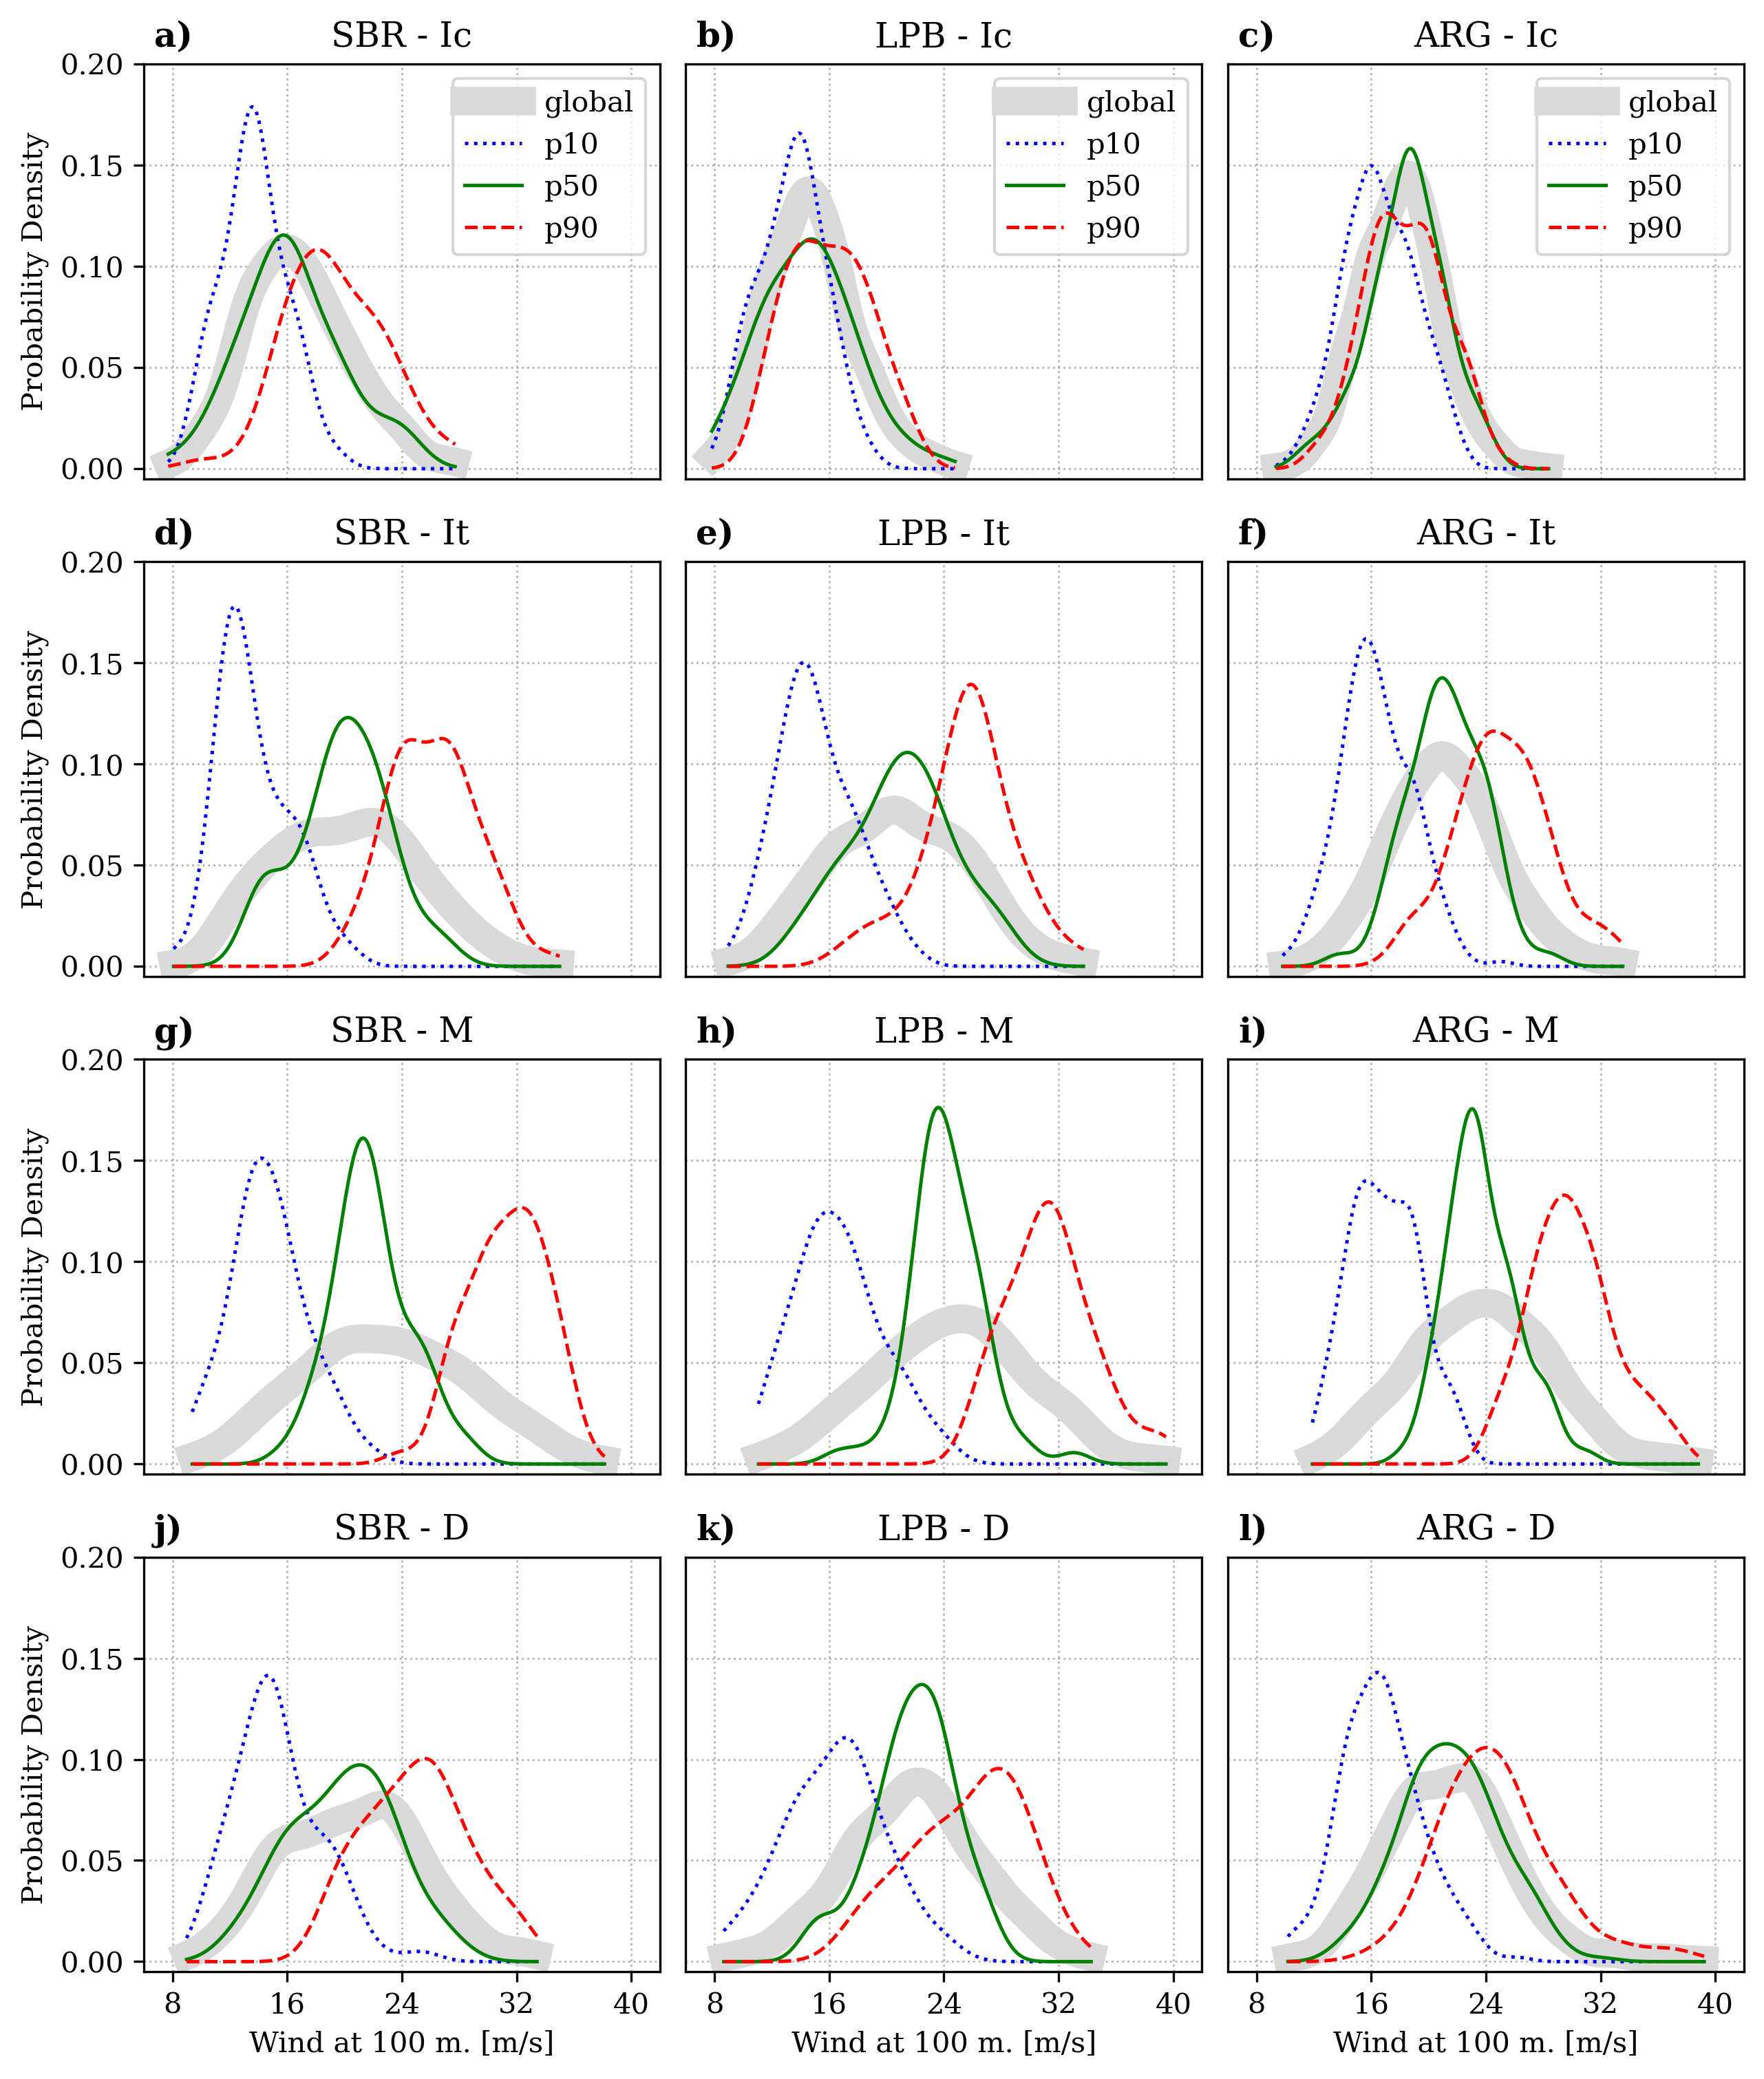
\includegraphics[width=\textwidth]{images/w100/PDF_wind100_sigma025.png}
\caption[PDF de magnitudes máximas de viento a 100 metros]{Estimación de las funciones de densidad de probabilidad (PDF) mediante la técnica de densidad por kernel para las magnitudes máximas del viento a 100 metros de altura. La matriz de paneles organiza la evolución temporal en filas, correspondientes a las fases de desarrollo evolutivo: Incipiente (a-c), Intensificación (d-f), Madurez (g-i) y Decaimiento (j-l). Las columnas separan la muestra según la región de ciclogénesis (SBR, LPB y ARG). Se contrasta la distribución de la Población Global de referencia (sombreado gris) frente a los estratos definidos por el pico máximo de vorticidad en su ciclo vital: sistemas débiles (p10, línea punteada azul), sistemas moderados (p50, línea continua verde) y sistemas extremos (p90, línea seccionada roja).}
\label{fig:pdf_wind100}
\end{figure}

La Figura \ref{fig:pdf_wind100} expone las funciones de densidad de probabilidad (PDF) para los valores máximos del campo de viento a 100 metros de altitud. De manera análoga al análisis de superficie, estos valores fueron extraídos del dominio lagrangiano de $20^\circ \times 20^\circ$ anclado al núcleo ciclónico. La muestra se evalúa a través de las cuatro fases del ciclo de vida y las tres regiones de génesis, contrastando el comportamiento estadístico de la Población Global frente a los estratos de intensidad dinámica (p10, p50 y p90).

El rasgo morfológico más sobresaliente al elevar el nivel de análisis a 100 metros es el corrimiento de todo el espectro probabilístico hacia magnitudes superiores y una separación inter-estrato significativamente más pronunciada que la observada a 10 metros. Durante la fase incipiente (paneles a-c), las distribuciones de todos los grupos presentan una estructura unimodal altamente superpuesta, con frecuencias máximas concentradas entre los 14 y 18 m/s. 

Sin embargo, a medida que los sistemas maduran (paneles g-i), la divergencia estructural se vuelve extrema. Mientras que el estrato moderado (p50) localiza su pico de máxima probabilidad en torno a los 20 m/s, la curva del subconjunto extremo (p90) experimenta un desplazamiento drástico hacia la derecha. En las regiones de LPB (h) y ARG (i), el grupo p90 alcanza modas entre 25 y 28 m/s, desarrollando colas pesadas de probabilidad que invaden el régimen de 32 a 40 m/s, revelando una alta dispersión intra-grupo hacia valores críticos. Durante el decaimiento (paneles j-l), las curvas extremas se aplanan levemente, denotando la relajación gradual del gradiente de presión, pero conservando una separación inconfundible respecto a la población moderada.

Desde el punto de vista físico, la amplificación de las magnitudes absolutas y el ensanchamiento de la brecha entre los estratos obedece al desacoplamiento parcial de la fricción superficial. A 100 metros de altura, en la cima de la capa de Ekman, el flujo se encuentra considerablemente menos atenuado por la rugosidad aerodinámica del océano o el continente. Esto permite que el intenso gradiente horizontal de presión que caracteriza a los vórtices severos \citep{reboita2010south} se exprese cinemáticamente con velocidades más cercanas al equilibrio geostrófico. En el caso particular de ARG, la prevalencia de vientos extremos con colas pesadas en el p90 refleja, además, un acoplamiento profundo con las anomalías cinemáticas asociadas al chorro polar de niveles superiores durante la fase de máxima baroclinicidad, un rasgo evolutivo detallado por \citet{hoskins2005new}.

Desde una perspectiva aplicada, la cuantificación de estas distribuciones en la capa límite superior tiene implicancias directas para la evaluación de cargas estructurales en la ingeniería eólica, dado que los 100 metros coinciden con la altura típica del buje en los aerogeneradores modernos. La evidencia estadística demuestra que el riesgo cinemático en estas altitudes no puede estimarse adecuadamente a partir de poblaciones medias o sistemas moderados (p50), ya que los ciclones clasificados dinámicamente como extremos (p90) originados en LPB o ARG superan con alta probabilidad los 30 m/s, generando escenarios de estrés mecánico que exigen umbrales de seguridad diferenciados.

% ==============================================================================
% SECCIÓN PRINCIPAL: KDE ESPACIAL DE VIENTO A 100 METROS
% ==============================================================================
%
\section{Distribución espacial de máximos de viento a 100 metros: Población global}\label{sec:kde_espacial_wind100_global}

\begin{figure}[htbp]
\centering
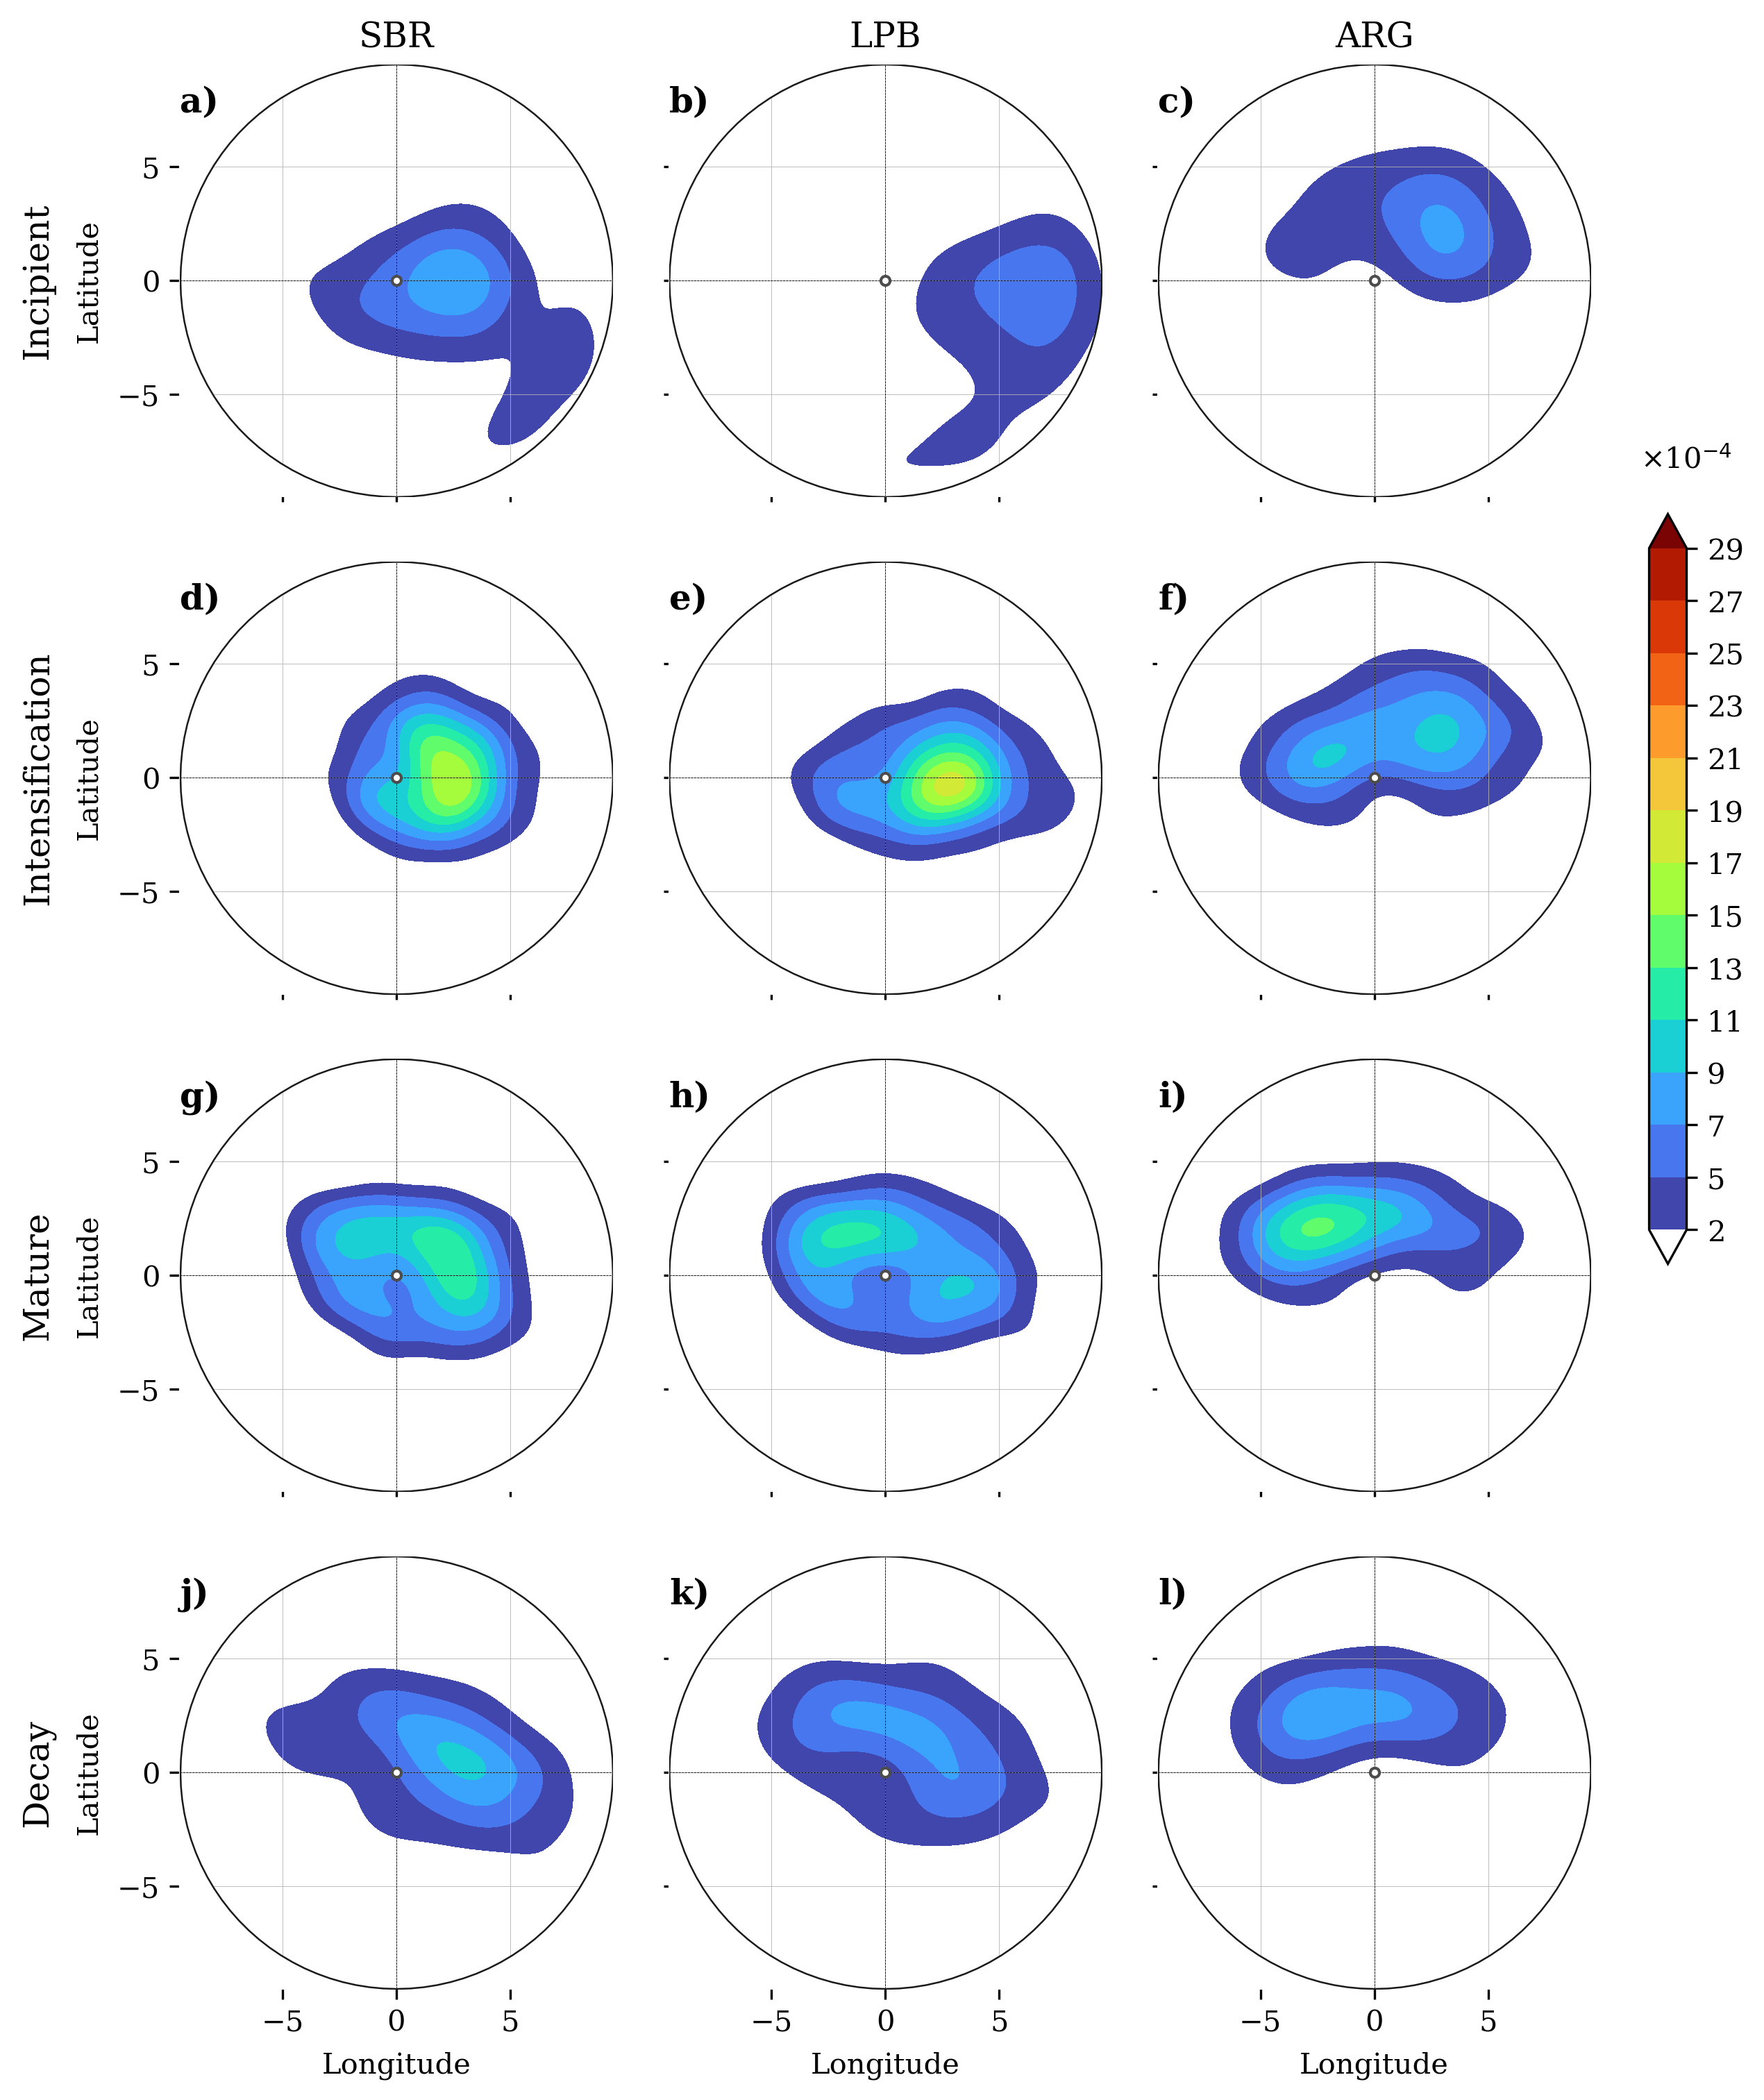
\includegraphics[width=\textwidth]{images/w100/kde_wind100_global_fasesxreg.png}
\caption[Distribución espacial (KDE) de viento máximo a 100 m - Población Global]{Estimación de densidad espacial bidimensional (KDE) para la ubicación geométrica de los máximos de magnitud del viento a 100 metros de altura en la Población Global de referencia. La matriz organiza la evolución espacial a través de las fases evolutivas Incipiente (a-c), Intensificación (d-f), Madurez (g-i) y Decaimiento (j-l), segregadas por las regiones de ciclogénesis SBR, LPB y ARG. El dominio lagrangiano abarca $20^{\circ} \times 20^{\circ}$ con centro en el núcleo del sistema $(0,0)$. La barra de colores cuantifica la densidad de probabilidad relativa escalada por $10^{-4}$.}
\label{fig:kde_wind100_global}
\end{figure}

La Figura \ref{fig:kde_wind100_global} presenta el campo probabilístico continuo, derivado de la estimación de densidad por kernel, que describe la ubicación espacial preferencial de los picos de viento a 100 metros de altura. Este análisis se aplica sobre la Población Global (población base) en un marco de referencia móvil anclado al centro de bajas presiones, trazando la evolución topológica del impacto cinemático en función de la región de ciclogénesis y su maduración a lo largo de las cuatro fases del ciclo de vida.

Al promediar el catálogo climatológico completo, la distribución espacial de los máximos a 100 metros mantiene una firma predominantemente difusa, amplia y con gradientes de probabilidad suaves a lo largo de su evolución. En las etapas iniciales (Ic; paneles a-c), la localización del viento máximo carece de un anclaje organizativo claro, presentando extensiones amplias e incluso zonas de densidad separadas, como se observa al sureste del centro en la región LPB (panel b). A medida que los ciclones avanzan hacia las etapas de intensificación y madurez (M; paneles g-i), el campo converge paulatinamente hacia el sector oeste y noroeste del núcleo ciclónico, estabilizándose no obstante en densidades de rango medio (valores entre 9 y $15 \times 10^{-4}$). Al ingresar en la fase de decaimiento (D; paneles j-l), esta incipiente organización se relaja, expandiendo nuevamente el área de dispersión de probabilidad sobre el cuadrante occidental.

Desde una perspectiva física, esta alta dispersión geométrica obedece a la vasta heterogeneidad estructural resultante de promediar un catálogo masivo dominado por ciclones ordinarios y someros. En sistemas con un forzamiento dinámico débil, la configuración del campo de viento depende fuertemente de la variabilidad del flujo sinóptico de fondo \citep{sinclair1994objective, hoskins2005new}. La leve consolidación temporal hacia el sector oeste y noroeste durante la madurez refleja la huella aerodinámica típica del sector frío post-frontal, donde el gradiente isobárico suele ser más pronunciado. Sin embargo, aunque a 100 metros de altura la fricción superficial es marginal, la carencia de una arquitectura termodinámica excepcionalmente profunda en el ciclón promedio impide que el flujo casi geostrófico se concentre en un único punto focal, resultando en un mapa de probabilidades altamente diluido.

La caracterización de esta distribución establece la línea base estructural probabilística para la cima de la capa límite. Al demostrar estadísticamente que un catálogo promediado de eventos no posee una simetría geométrica rígida ni un punto de impacto altamente predecible, se justifica la necesidad metodológica de estratificar la muestra por intensidad, un enfoque sistemático indispensable para aislar la minoría de eventos severos de la variabilidad media \citep{corner2025classification, eisenstein2023identification}. En el contexto de la evaluación de recursos eólicos y diseño estructural costa afuera, este patrón medio confirma que, bajo condiciones climatológicas normales, la energía cinética extrema se encuentra distribuida de manera variable, proporcionando el sustrato necesario para contrastar y dimensionar posteriormente la hiperconcentración topológica asociada a los estratos de gran severidad.
%%
%%%%
%%%%%%
%%%%
%%
\section{Distribución espacial de máximos de viento a 100 metros: Subconjunto extremo (p90)}\label{sec:kde_espacial_wind100_p90}

\begin{figure}[htbp]
\centering
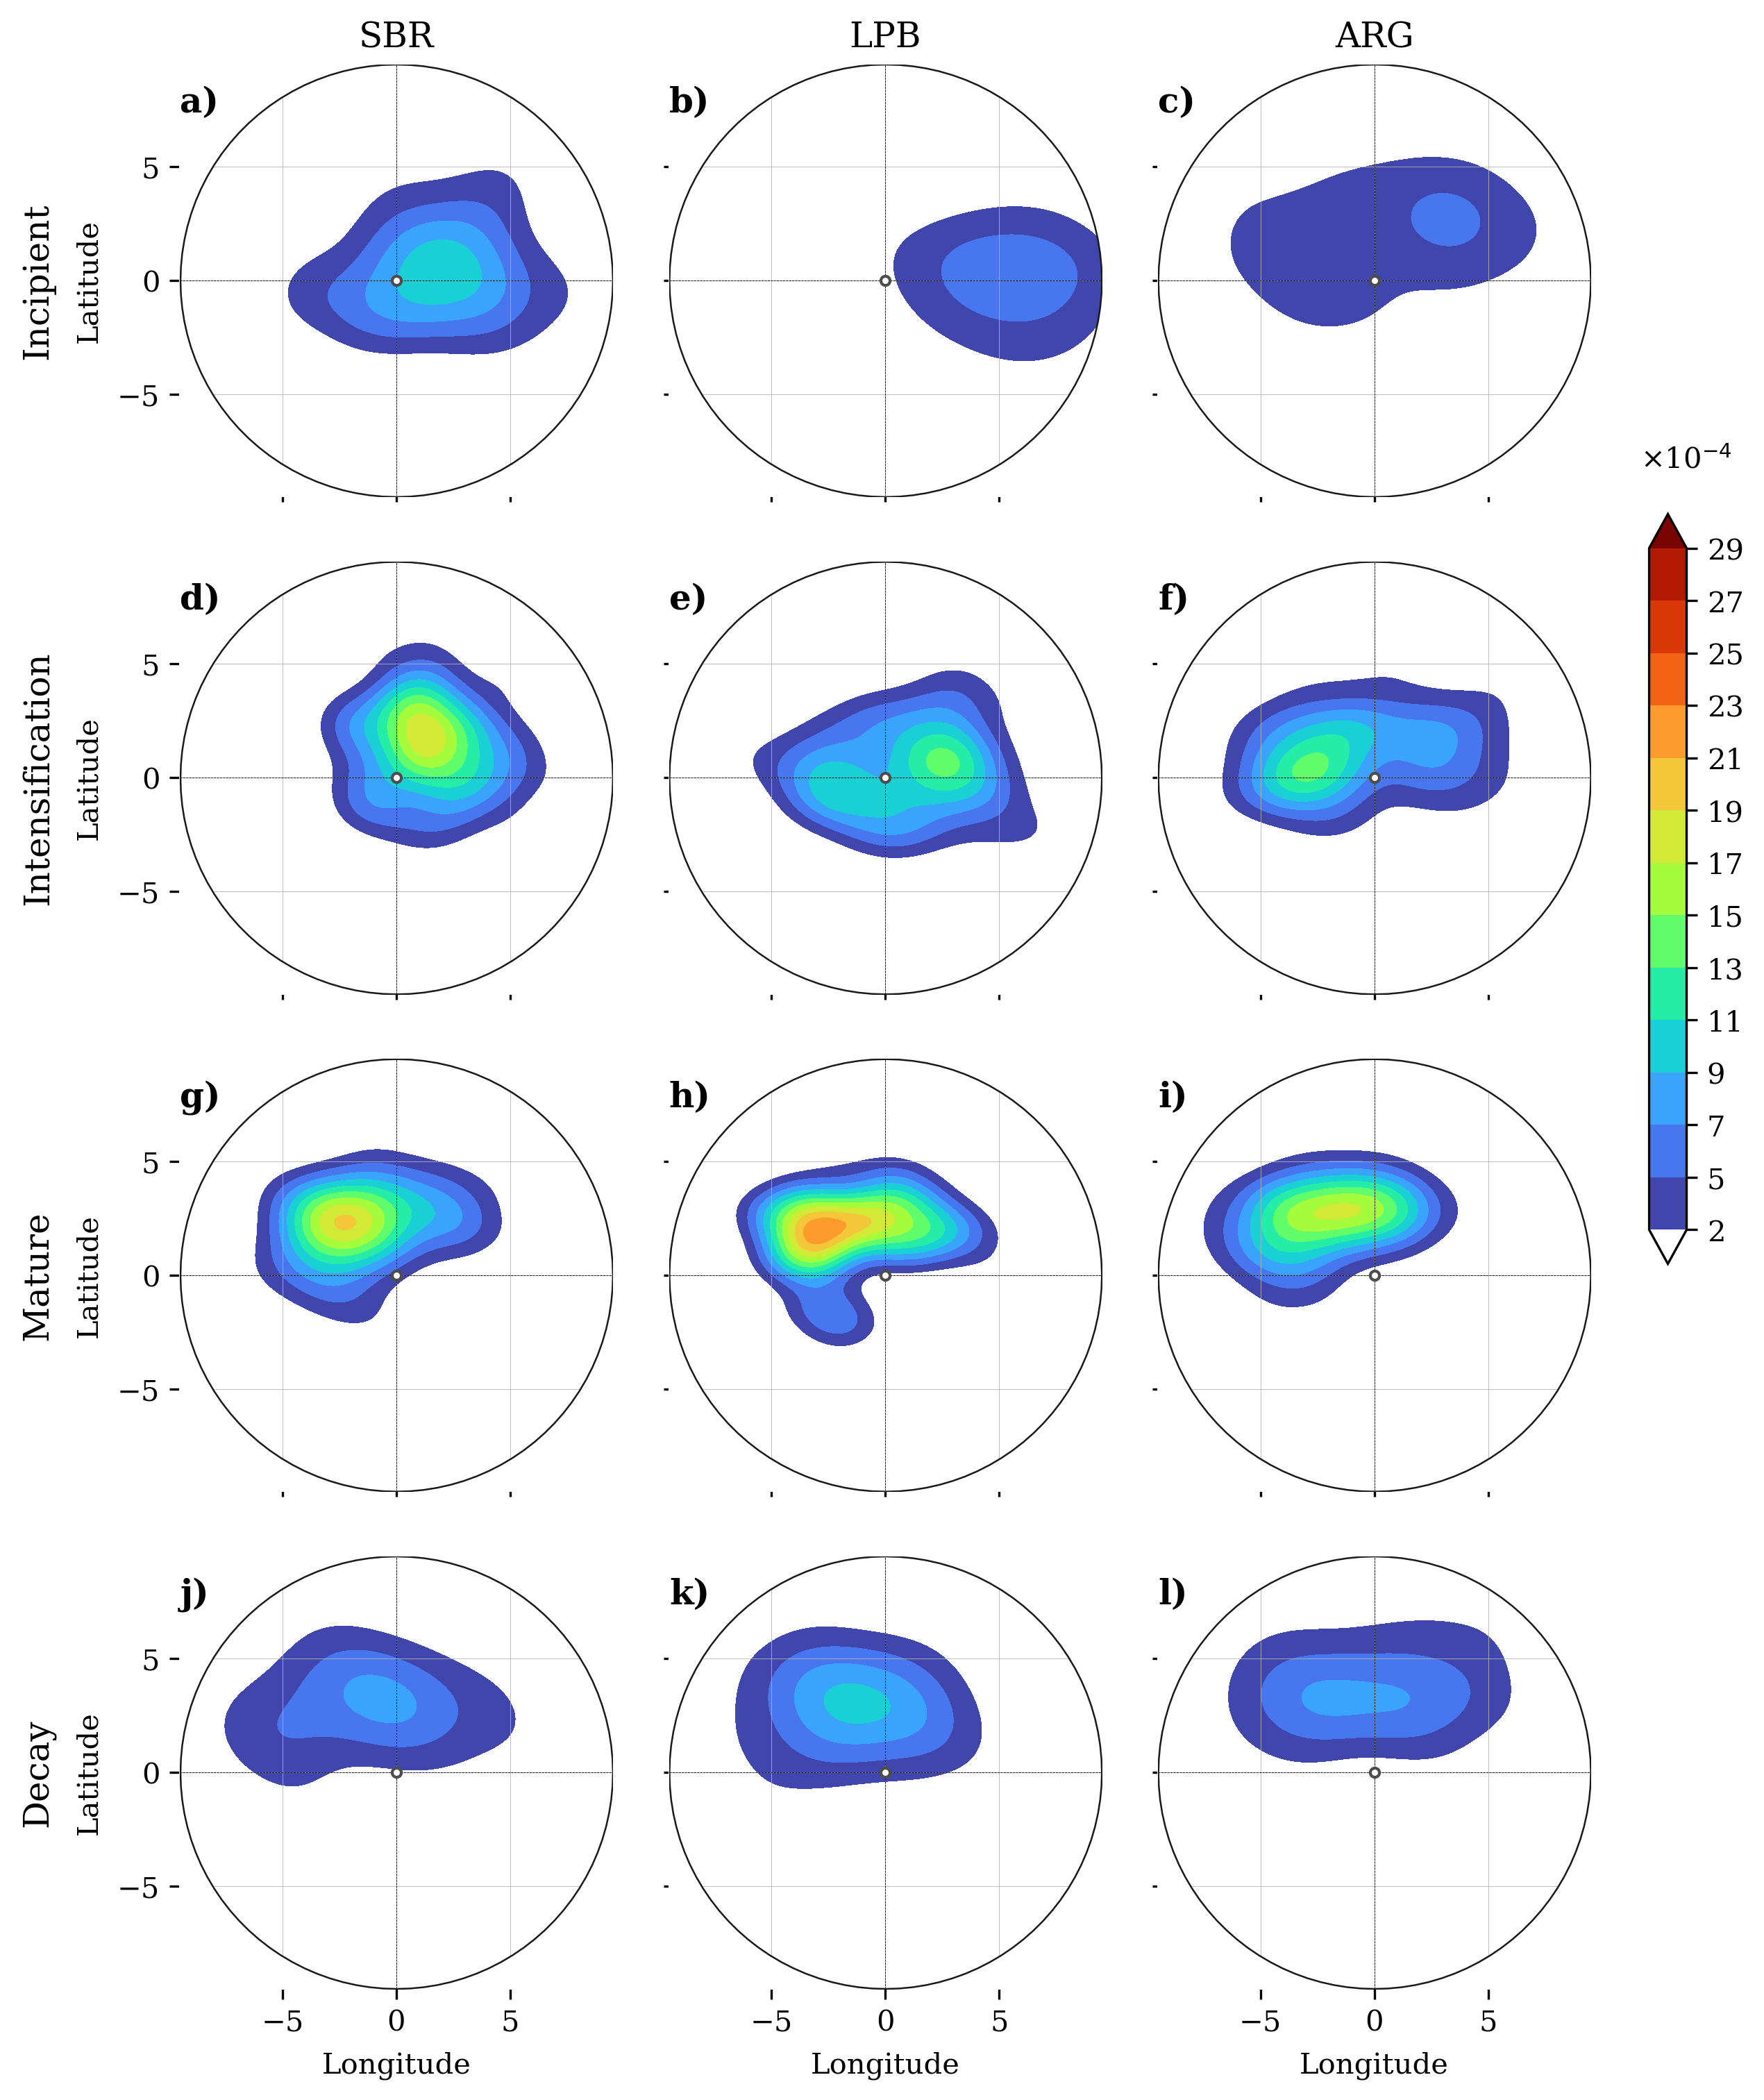
\includegraphics[width=\textwidth]{images/w100/kde_wind100_p90_fasesxreg.png}
\caption[Distribución espacial (KDE) de viento máximo a 100 m - Subconjunto p90]{Estimación de densidad espacial bidimensional (KDE) de la ubicación de los máximos de magnitud del viento a 100 metros para el subconjunto de ciclones intensos (percentil 90). La disposición de los paneles (a-l) y el formato del dominio lagrangiano replican a la Figura \ref{fig:kde_wind100_global}, empleando la misma escala colorimétrica ($10^{-4}$) para evidenciar el agudo contraste en la concentración y previsibilidad del impacto cinemático en eventos extremos.}
\label{fig:kde_wind100_p90}
\end{figure}

La Figura \ref{fig:kde_wind100_p90} presenta el modelado espacial KDE enfocado exclusivamente en el estrato de ciclones extremos (percentil 90). Esta muestra aísla la firma geométrica de los vientos máximos a 100 metros de altitud para los vórtices dinámicamente más severos del catálogo, aquellos que durante su ciclo vital alcanzaron los valores de vorticidad relativa a 850 hPa correspondientes al primer decil de la distribución. El análisis desglosa la evolución de esta arquitectura cinemática a través de las fases de desarrollo y los tres principales focos ciclogenéticos.

A diferencia de la amplia dispersión observada en la climatología media, el campo probabilístico del estrato p90 exhibe una contracción topológica drástica. Al alcanzar la fase de madurez (M; paneles g-i), se configura un núcleo hiperlocalizado de máxima densidad anclado sólidamente en el cuadrante noroeste del sistema. En las regiones de SBR (g) y LPB (h), el epicentro de este núcleo satura la escala de probabilidad (tonos cálidos, superando los $23 \times 10^{-4}$), denotando una recurrencia espacial altísima. En ARG (i), el patrón es análogamente coherente, aunque ligeramente más elongado sobre el eje zonal. De manera notable, al transitar hacia el decaimiento (D; paneles j-l), los sistemas del p90 conservan una estructura espacial significativamente más compacta y confinada cerca del núcleo que su contraparte de la Población Global.

Esta marcada concentración geométrica demuestra que, en sistemas extremos, la intensa rotación cerrada de mesoescala domina y suprime la dispersión topológica generada por el flujo ambiental de fondo. Desde el punto de vista físico, el desacoplamiento parcial de la fricción superficial a 100 metros de altura facilita que las estructuras dinámicas severas operen sin las atenuaciones mecánicas presentes cerca del suelo. Como indican \citet{clark2005sting} y \citet{han2025system}, en los ciclones más profundos, los vientos extremos se asocian a las intensas corrientes en chorro de niveles bajos y a la cinta transportadora fría (\textit{cold conveyor belt}), las cuales se envuelven en el sector posterior del frente frío. Por efecto de la circulación horaria en el Hemisferio Sur, esta dinámica frontal se posiciona en el cuadrante noroeste, coincidiendo exactamente con la máxima densidad revelada por el KDE. 

Las diferencias de agudeza interregional respaldan este marco conceptual. Los desarrollos originados en SBR y LPB suelen adquirir arquitecturas más compactas (seclusiones cálidas pronunciadas) promovidas por intensos flujos diabáticos desde el océano \citep{reboita2018extratropical, gramcianinov2023impact}, lo que permite empaquetar el gradiente de presión destructivo en un volumen espacial minúsculo. En contraposición, la dinámica baroclínica del frente polar en ARG genera estructuras marginalmente más elongadas.

La cuantificación geométrica de este núcleo asimétrico constituye un hallazgo importante para la estimación de riesgos en infraestructuras elevadas, como los aerogeneradores marinos. Demuestra concluyentemente que el grado de severidad dinámica de un ciclón predetermina su coherencia espacial, forzando a que las ráfagas extremas a 100 metros se sistematicen en un sector específico y predecible. Para la meteorología operativa y la ingeniería eólica, esto implica que, al identificar un sistema severo en desarrollo, el sector de mayor impacto aerodinámico puede anticiparse con un elevado grado de certidumbre espacial, permitiendo optimizar medidas operativas preventivas (como la puesta en bandera o \textit{pitching} de las aspas) frente a cargas estructurales críticas \citep{dalanhese2023new}.

% ==============================================================================
% SECCIÓN: PATRONES DOMINANTES DE VARIABILIDAD (EOF) - VIENTO A 10 METROS
% ==============================================================================
\section{Varianza explicada del Viento a 100 metros}\label{sec:var_exp_wind100}

\begin{figure}[!ht]
\centering
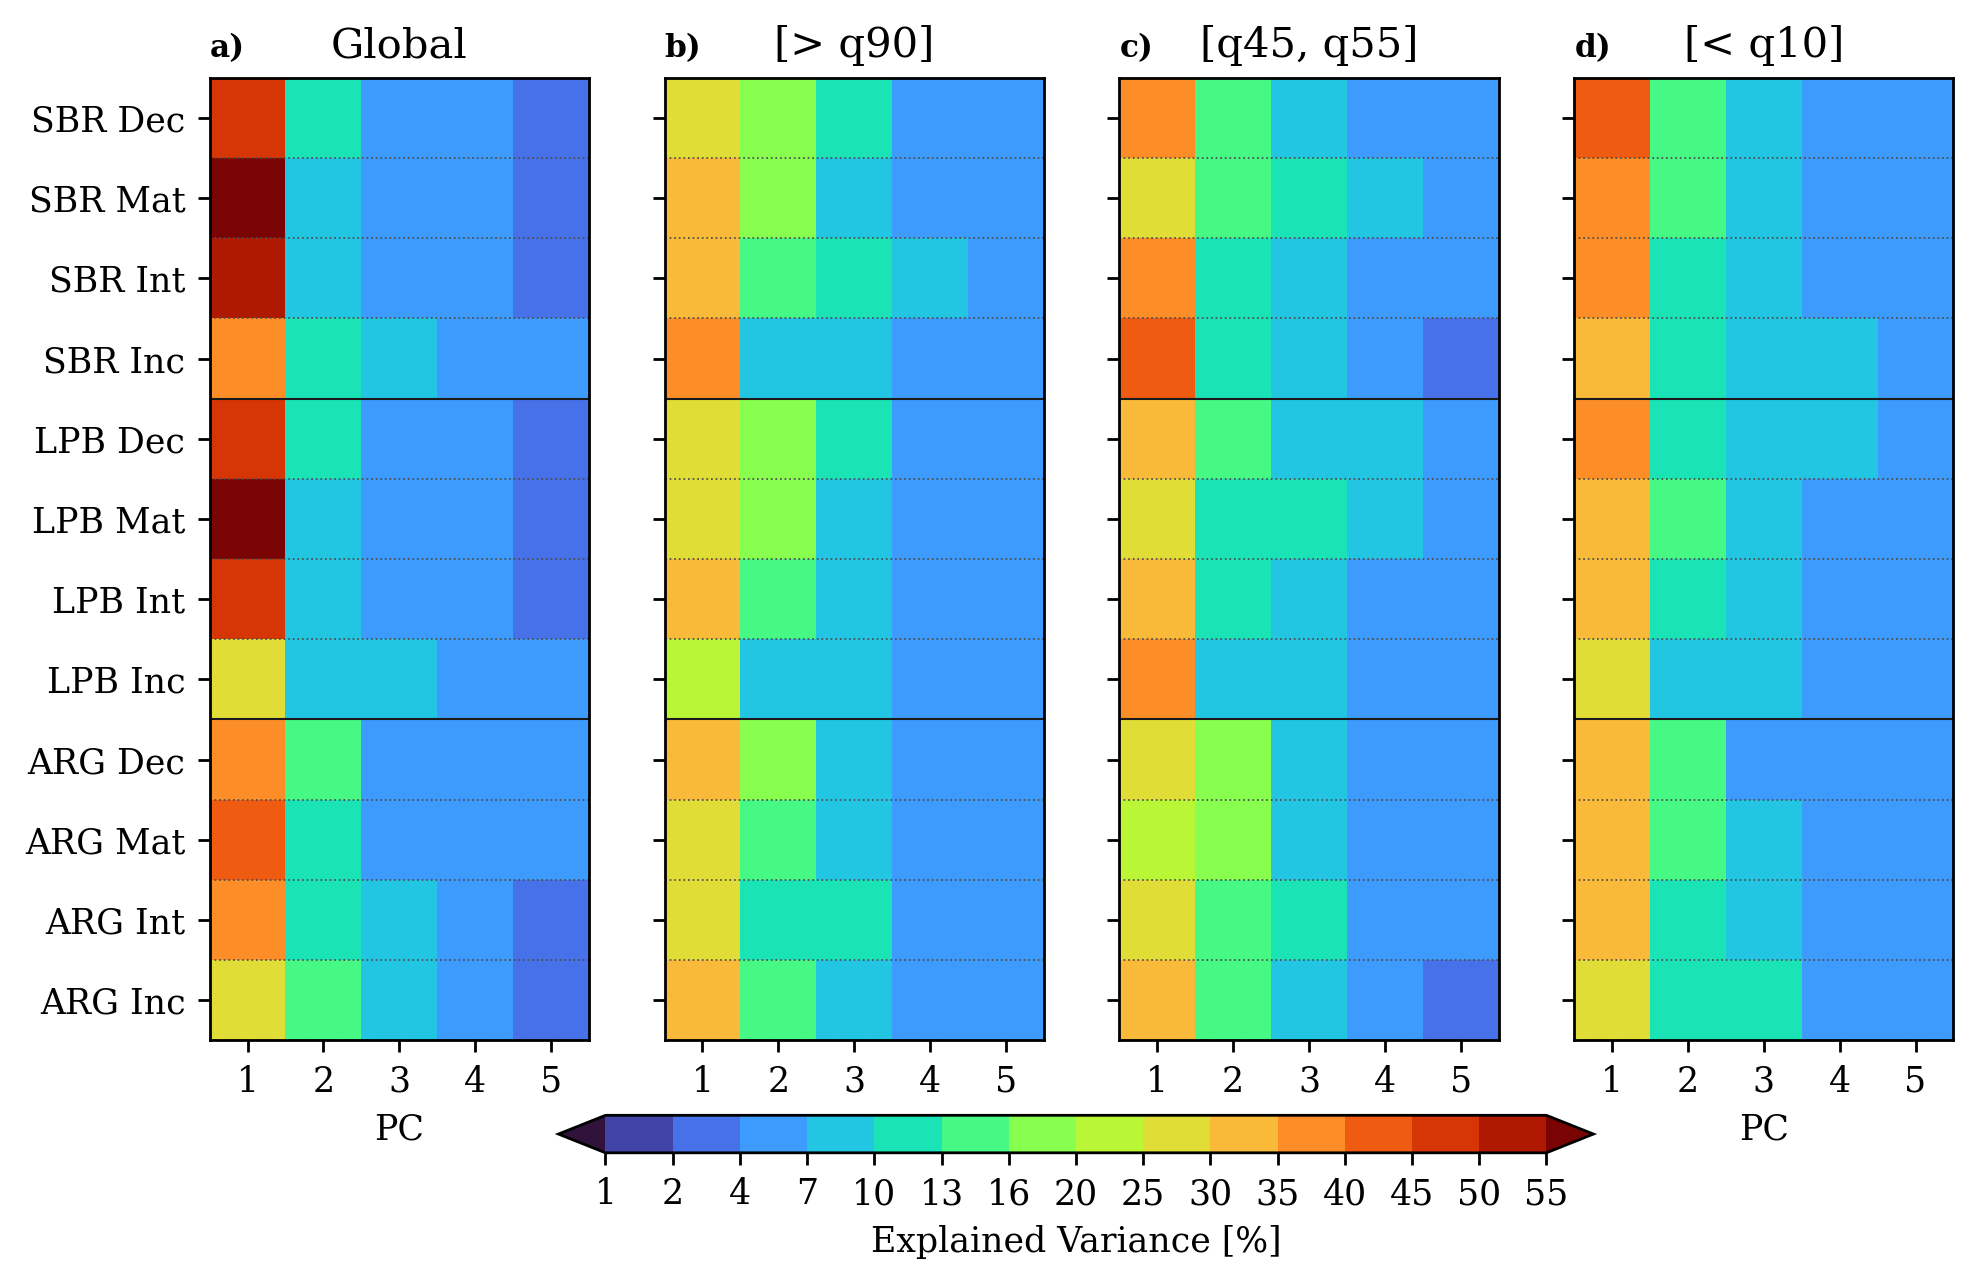
\includegraphics[width=\textwidth]{images/w100/all_expvar_wind100_mean2times.png} % Ajusta el nombre de tu archivo
\caption[Varianza explicada por los primeros cinco modos (EOF1-EOF5) de viento a 100 m]{Fraccionamiento de la varianza espacial total contenida en los primeros cinco modos dominantes (EOF1 a EOF5) del campo de viento a 100 metros de altura. Se contrasta la distribución de la Población Global frente a los estratos de intensidad (p10, p50 y p90) a lo largo del ciclo de vida para cada región de ciclogénesis.}
\label{fig:var_exp_wind100}
\end{figure}

La Figura \ref{fig:var_exp_wind100} sintetiza el fraccionamiento de la varianza espacial distribuida en los primeros cinco modos ortogonales (EOF1 a EOF5) del campo de viento a 100 metros de altura. Al igual que en el nivel superficial, este desglose permite evaluar la dimensionalidad y cohesión de la energía cinética, contrastando el comportamiento de la Población Global de referencia frente a los estratos de distinta intensidad dinámica intrínseca (p10, p50 y p90) a lo largo de las fases evolutivas.

El análisis revela que, a 100 metros de altitud, la dicotomía distributiva entre la población media y los eventos extremos se profundiza notablemente. En la Población Global, así como en los estratos de menor y media intensidad (p10 y p50), el modo EOF1 ejerce una clara dominancia, capturando entre el $28.9\%$ y el $58.6\%$ de la varianza espacial total. Esto genera un declive pronunciado hacia las componentes de orden superior (EOF2 a EOF5), las cuales retienen porciones marginales de energía. Por el contrario, al evaluar el estrato extremo (p90), la representatividad del primer modo colapsa matemáticamente, descendiendo a valores de entre $24.3\%$ y $38.0\%$. Consecuentemente, la varianza del p90 se redistribuye y aplana, inflando la importancia relativa de los modos ortogonales secundarios.

Desde el punto de vista físico, la alta concentración de energía en un solo modo (EOF1) para el grupo global corrobora que la circulación de los ciclones ordinarios obedece de manera estructurada al gradiente de gran escala impuesto por el flujo sinóptico de fondo, un efecto que se vuelve aún más nítido al desvincularse parcialmente de la capa límite friccional. Sin embargo, el aplanamiento de la varianza en los eventos severos (p90) evidencia un proceso dinámico de fragmentación multiescalar. Tal como establece la teoría matemática de \citet{hannachi2007empirical}, un espectro de autovalores más plano es el indicador de que la energía de un sistema complejo se ha distribuido entre múltiples modos competitivos. Al liberarse de la atenuación friccional cerca del suelo, la enorme inestabilidad del vórtice extremo facilita el desarrollo irrestricto de intensas perturbaciones internas no lineales, como corrientes en chorro de bajos niveles (\textit{low-level jets}) y fuertes gradientes asociados a oclusiones rápidas. Estas estructuras de mesoescala rompen el flujo univariado y compiten por la energía cinética del campo, obligando a la descomposición matemática a utilizar múltiples dimensiones espaciales para reconstruir la severidad cinemática del ciclón.

Esta métrica constituye una demostración cuantitativa de que los eventos extremos a 100 metros de altura requieren forzosamente de múltiples dimensiones ortogonales para ser explicados. Para la industria de las energías renovables, confirmar que la energía de un sistema p90 se reparte en múltiples patrones estructurales a la altura estándar del buje certifica que las cargas extremas de viento son espacialmente complejas y multiformes. Esto alerta a la ingeniería eólica sobre el sesgo que implica subestimar la fatiga aerodinámica: los modelos de evaluación de riesgo costa afuera deben incorporar parametrizaciones multiescalares capaces de soportar ráfagas hiperlocalizadas que cambian rápidamente de forma, descartando las proyecciones basadas en un único patrón espacial dominante.
%%
%%%%
%%%%%%
%%%%
%%
\section{Patrones de variabilidad del viento a 100 metros: EOF1 población global}\label{sec:eof1_wind100_global}

\begin{figure}[htbp]
\centering
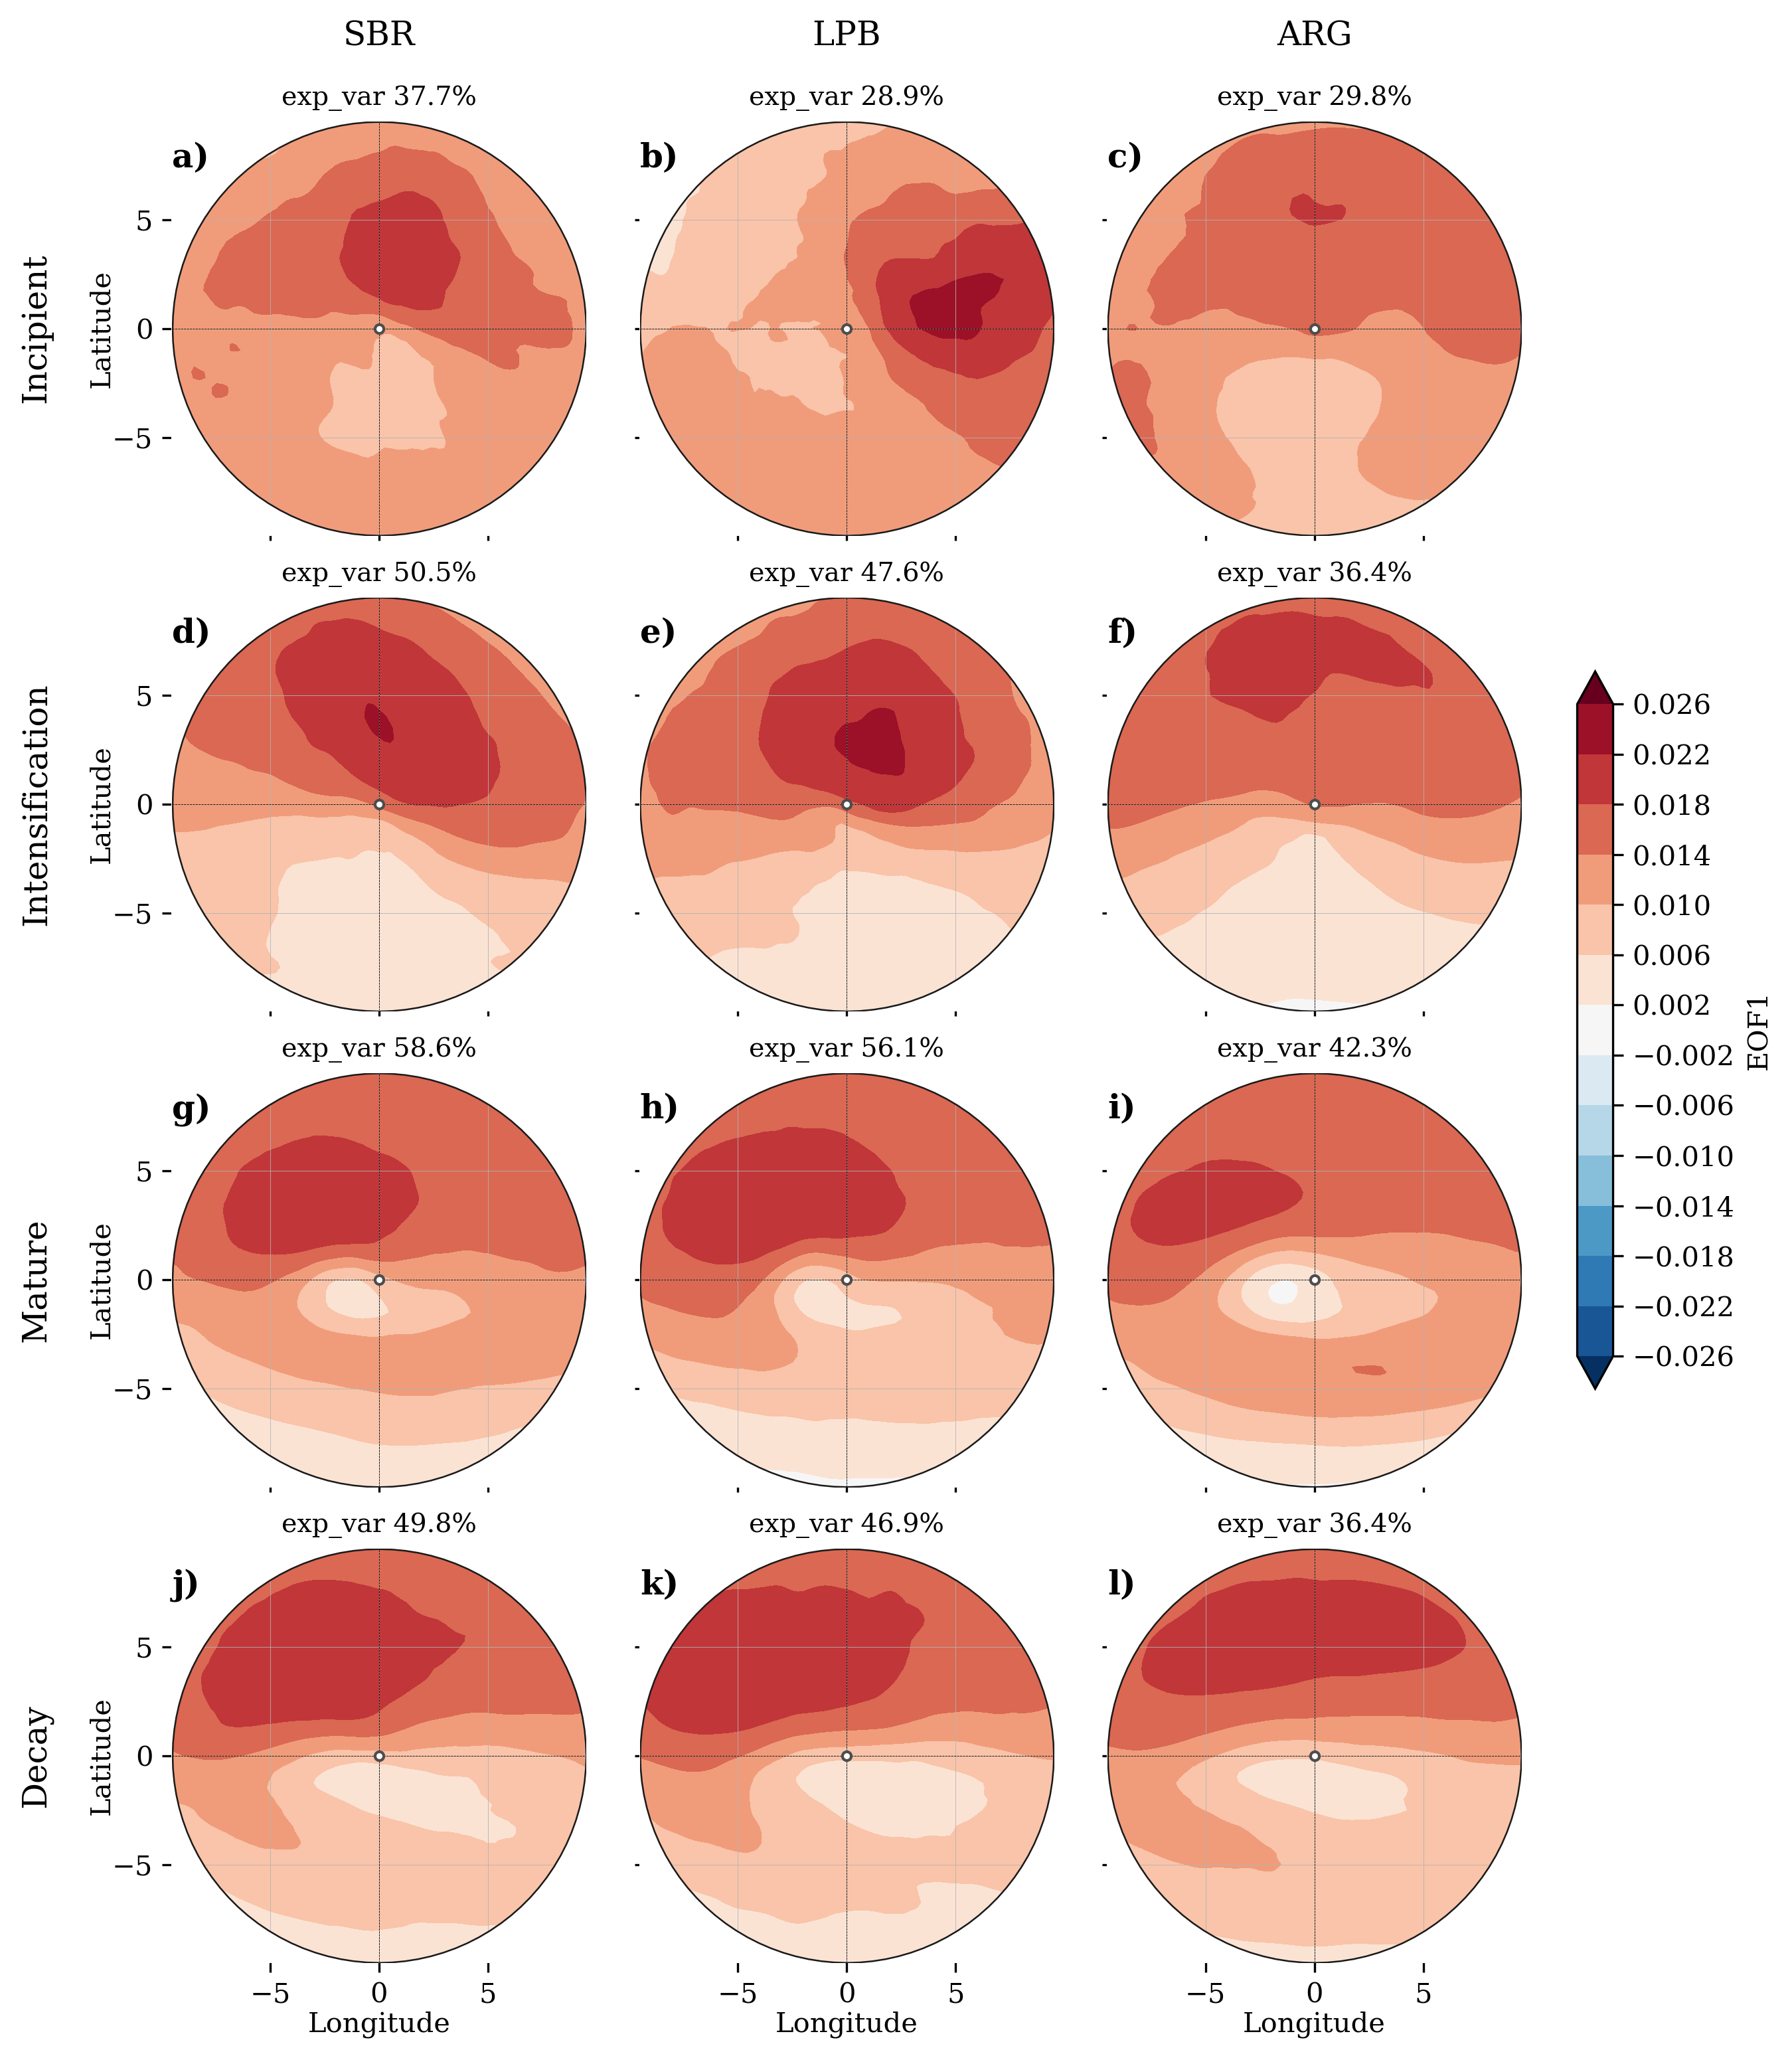
\includegraphics[width=\textwidth]{images/w100/pca1_wind100_global_fasesxreg.png}
\caption[EOF1 de viento a 100 metros - Población Global]{Primer modo espacial (EOF1) de la magnitud del viento a 100 metros para la Población Global de referencia. La disposición matricial organiza la evolución por regiones de ciclogénesis en columnas (SBR, LPB y ARG) y las fases de desarrollo evolutivo en filas (Incipiente, Intensificación, Madurez y Decaimiento), etiquetadas de la a) a la l). Sobre cada panel se indica el porcentaje de la varianza espacial total explicada (\textit{exp\_var}) por esta componente principal. La escala cromática divergente cuantifica las anomalías estructurales relativas al centro del vórtice.}
\label{fig:eof1_wind100_global}
\end{figure}

La Figura \ref{fig:eof1_wind100_global} presenta el primer modo de las Funciones Ortogonales Empíricas (EOF1) del campo de viento a 100 metros de altura. Este diagnóstico aísla matemáticamente la señal de variabilidad recurrente en la cima de la capa límite. El análisis se aplica sobre la Población Global y se estratifica por región de ciclogénesis y fase de desarrollo, permitiendo establecer la línea base aeroelástica estructural para el ciclón extratropical promedio a lo largo de su ciclo de vida.

Tal como se evidenció en el fraccionamiento de energía (Sección \ref{sec:var_exp_wind100}), el modo dominante EOF1 ejerce un control casi absoluto sobre la varianza del sistema medio, capturando entre el $28.9\%$ y el $58.6\%$ de la varianza total (alcanzando su máxima representatividad durante la madurez en la región SBR). Topológicamente, este patrón preserva e incluso amplifica la estructura dipolar de gran escala orientada meridionalmente que se observó en el nivel superficial, pero exhibiendo contornos espacialmente más suaves y bandas de anomalías mucho más expansivas.

Desde una perspectiva dinámica, la persistencia de este gran dipolo meridional con tan alta varianza explicada obedece a la naturaleza del flujo en niveles parcialmente desvinculados de la fricción superficial. Al promediar el comportamiento de miles de sistemas ordinarios a 100 metros de altura, las fluctuaciones cinemáticas dependen de manera casi exclusiva del flujo geostrófico de fondo. De acuerdo con los principios expuestos por \citet{hannachi2007empirical}, la emergencia de una estructura dipolar dominante en el primer modo espacial constituye la firma matemática del desplazamiento posicional de una corriente. En el contexto del Hemisferio Sur, estas anomalías reflejan los desplazamientos latitudinales del flujo del oeste y las expansiones del gradiente térmico en las zonas baroclínicas \citep{hoskins2005new, dossantos2023response}. 

La extracción de este patrón continuo en la capa límite superior sirve para identificar que la fluctuación principal en los ciclones ordinarios obedece a un dipolo meridional impulsado por el entorno sinóptico permite separar matemáticamente las alteraciones inducidas por la corriente de fondo de aquellas generadas por la propia inestabilidad interna del vórtice. Este contraste climatológico sirve como el marco de referencia exacto para demostrar, en el análisis subsiguiente, cómo los eventos extremos fracturan esta simetría geostrófica y organizan su momento cinético en estructuras de mesoescala completamente asimétricas.
%%
%%%%
%%%%%%
%%%%
%%
\section{Patrones dominantes de variabilidad del viento a 100 metros: EOF1 Subconjunto extremo (p90)}\label{sec:eof1_wind100_p90}

\begin{figure}[htbp]
\centering
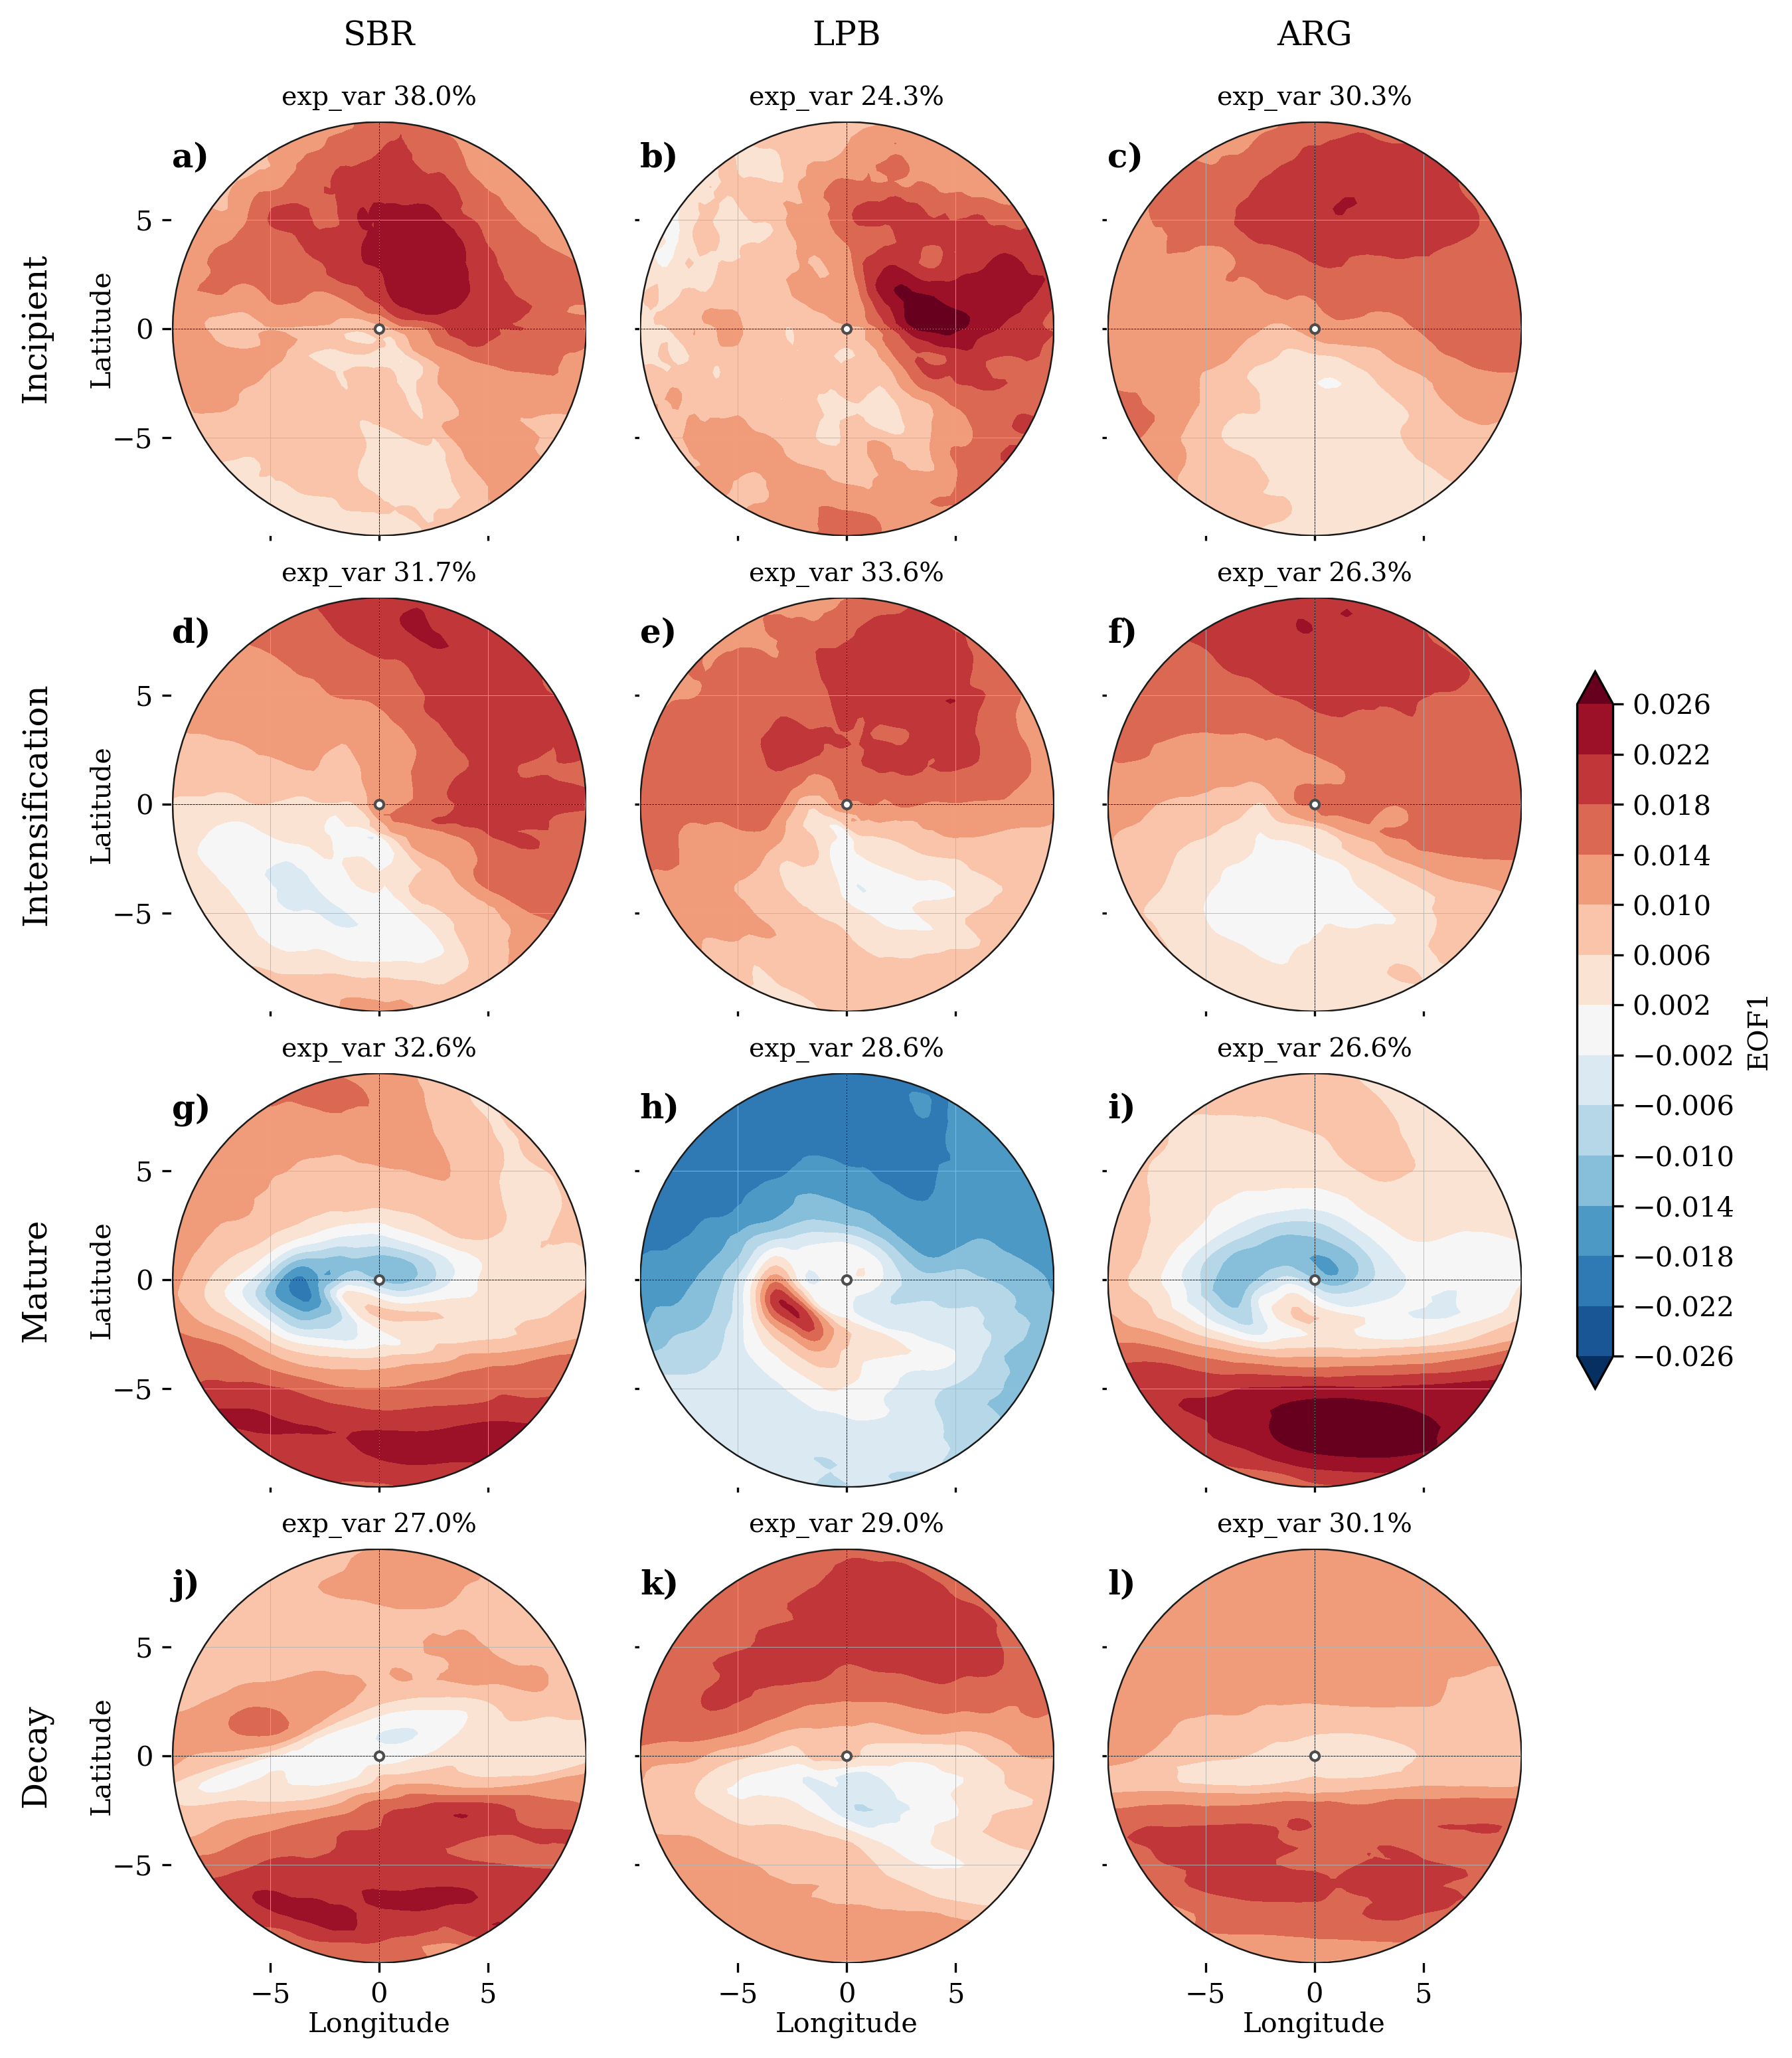
\includegraphics[width=\textwidth]{images/w100/pca1_wind100_p90_fasesxreg.png}
\caption[EOF1 de viento a 100 metros - Subconjunto p90]{Primer modo espacial (EOF1) de la magnitud del viento a 100 metros para el estrato de ciclones extremos (percentil 90). El formato de los paneles (a-l), la nomenclatura de varianza explicada y el dominio espacial mantienen una correspondencia estricta con la Figura \ref{fig:eof1_wind100_global}, permitiendo el contraste topológico directo entre la dinámica intrínseca de los sistemas severos y el patrón climatológico medio.}
\label{fig:eof1_wind100_p90}
\end{figure}

La Figura \ref{fig:eof1_wind100_p90} ilustra la primera Función Ortogonal Empírica (EOF1) calculada exclusivamente a partir de los campos espaciales a 100 metros de altura para el subconjunto de ciclones extremos (percentil 90). Este análisis aísla las fluctuaciones dominantes en la capa límite superior para los sistemas con mayor severidad dinámica (vorticidad relativa mínima en el primer decil). Tal como se anticipó en el fraccionamiento de la varianza (Sección \ref{sec:var_exp_wind100}), la proporción de energía capturada por el modo EOF1 se reduce drásticamente frente a la población global, oscilando entre el $24.3\%$ y el $38.0\%$.

En consonancia con esta caída matemática, la topología del modo dominante difiere radicalmente de la estructura suave observada en la climatología media: el patrón dipolar expansivo se fractura y da paso a firmas espacialmente complejas e hiperlocalizadas. En la fase de madurez de la región LPB (panel h), emerge un núcleo de anomalía positiva excepcionalmente denso, compacto y elongado hacia el sur y sureste del centro (tonos rojo oscuro, $>+0.04$). Por su parte, la región ARG en madurez (panel i) desarrolla una compleja firma asimétrica con gradientes agudos en torno al núcleo. Al ingresar al decaimiento (paneles j-l), las bandas anómalas de los sistemas p90 permanecen fuertemente ancladas y compactadas alrededor del vórtice, configurando gradientes espaciales mucho más agresivos que la relajación estrictamente zonal de la población general.

Físicamente, la quiebra del patrón dipolar simple y la hiperconcentración de anomalías evidencian que, bajo un forzamiento dinámico extremo a 100 metros de altura, la arquitectura interna del vórtice toma el control absoluto, anulando la influencia del flujo de fondo. Al operar cerca del tope de la capa de Ekman, libres de la atenuación y disipación friccional mecánica presente en superficie, las estructuras mesoescalares logran expresarse en su máxima magnitud. De acuerdo con \citet{clark2005sting} y \citet{han2025system}, la hiperconcentración de variabilidad en los sectores posteriores y polares es la firma espacial inconfundible de inestabilidades agudas en la cinta transportadora fría (\textit{cold conveyor belt}) y en las corrientes en chorro de bajo nivel asociadas a la fractura frontal rápida. Asimismo, patrones espacialmente complejos y anulares como el de ARG responden a fluctuaciones en el tamaño de la seclusión cálida (\textit{warm seclusion}) del modelo de Shapiro-Keyser, un rasgo típico de sistemas oceánicos altamente organizados \citep{schultz2021antecedents, reboita2022from}.

La cuantificación de estos modos revela una conclusión central que hace eco de lo observado a 10 metros, pero con implicancias estructurales mucho más críticas: un ciclón extremo no es equivalente a un ciclón ordinario escalado linealmente \citep{corner2025classification, eisenstein2023identification}. Extraer estas firmas asimétricas en la capa límite superior es importante en la estimación de riesgos en infraestructuras. Demostrar estadísticamente que un estrato de vórtices extremos no solo incrementa su velocidad escalar, sino que fractura y concentra su varianza en núcleos hipercompactos, permite refinar de manera determinística la modelación de fatiga aerodinámica sobre los rotores de las turbinas eólicas. Esto ratifica que los códigos de diseño ingenieril deben incorporar forzosamente la dimensionalidad asimétrica de la mesoescala para prever los impactos reales, descartando la premisa de que la amenaza cinemática extrema a 100 metros se distribuye de manera concéntrica o gobernada por un único patrón espacial.